%%
%% kit-prog-tutorial
%%
%% Slides for my Java programming tutorial at KIT using LaTeX beamer.
%%
%% Copyright (c) 2015-2016 YouniS Bensalah <younis.bensalah@gmail.com>
%%
%% This work is released to the public domain.
%% For the full copyright and license information, please view the LICENSE file.
%%

\documentclass[18pt]{beamer}

\usepackage{templates/beamerthemekit}

\usepackage[utf8]{inputenc}
\usepackage{hyperref}
\usepackage{listings}
\usepackage{xcolor}
\usepackage{colortbl}

\titleimage{road}

\definecolor{lime}{HTML}{8FFF53}

\newcommand{\tagline}{Conversion, Visibility, Arrays}

\newcommand{\quotes}[1]{``#1''}

\title[Programmieren\hspace{2.5pt}--\hspace{2.5pt}\tagline]{\tagline}
\subtitle{Programmieren~\textbar~Tutorium 32}

\author{YouniS Bensalah}
\date{28. November 2016}

\institute{Chair for Software Design and Quality}

\usepackage[citestyle=authoryear,bibstyle=numeric,hyperref,backend=biber]{biblatex}
\addbibresource{templates/example.bib}
\bibhang1em

\begin{document}

% remove annoying figure prefix in caption
\setbeamertemplate{caption}{\raggedright\insertcaption\par}

\selectlanguage{english}

\begin{frame}
    \titlepage
\end{frame}

% \begin{frame}{Heute}
%     \tableofcontents
% \end{frame}

\section{Typ-Konvertierung}

\begin{frame}{Typ-Konvertierung}
    \begin{itemize}
        \item Was passiert, wenn ich einen Datentyp in einen anderen umwandele?
    \end{itemize}
\end{frame}

\begin{frame}[fragile]{Widening Primitive Conversions}
    \begin{itemize}
        \item Beispiel: von \texttt{int} nach \texttt{float}
        \item Kein Informationsverlust bzgl. \textbf{Größe}
        \item Informationsverlust bzgl. \alert{\textbf{Präzision}} möglich
        \item Automatisch: kein expliziter Cast erforderlich
        \begin{lstlisting}[language=Java]
int big = 1111111111;
float approx = big; // int to float
System.out.println((int)approx); // 1111111168
        \end{lstlisting}
    \end{itemize}
\end{frame}

\begin{frame}[fragile]{Narrowing Primitive Conversions}
    \begin{itemize}
        \item Beispiel: von \texttt{int} nach \texttt{byte}
        \item Informationsverlust bzgl. \alert{\textbf{Größe}} möglich
        \item Informationsverlust bzgl. \alert{\textbf{Präzision}} möglich
        \item Bei ganzzahligen Typen werden höherwertige Bits einfach abgeschnitten
        \item \textbf{Cast-Operator} notwendig
        \begin{lstlisting}[language=Java]
int x = 2000;
System.out.println((byte)x); // -48
        \end{lstlisting}
    \end{itemize}
\end{frame}

\begin{frame}[fragile]{String Conversions}
    \begin{itemize}
        \item Jeder Datentyp kann nach String konvertiert werden
        \item Für primitive Typen geschieht dies automatisch
        \item Für Klassen kann man eine eigene \texttt{toString} Methode angeben
        \begin{lstlisting}[language=Java]
class Vector2D {
    double x, y;

    public String toString() {
        return "(" + x + ", " + y + ")";
    }
}
        \end{lstlisting}
    \end{itemize}
\end{frame}

\section{Sichtbarkeit}

\begin{frame}{Sichtbarkeit: \texttt{public} und \texttt{private}}

    \begin{itemize}
        \item \texttt{public} und \texttt{private} sind Sichtbarkeitsmodifizierer
        \item Sichtbarkeitsmodifizierer können auf \textbf{Attribute}, \textbf{Methoden} und \textbf{Klassen} angewandt werden
        \item \texttt{public}
        \begin{itemize}
            \item Nach außen sichtbar
        \end{itemize}
        \item \texttt{private}
        \begin{itemize}
            \item Nur von innen sichtbar
        \end{itemize}
    \end{itemize}
\end{frame}

\begin{frame}{Datenkapselung}
    \begin{itemize}
        \item Verbergen von Details einer Klasse
        \item Details der Implementierung nicht nach außen sichtbar
        \item Weniger Abhängigkeiten zwischen Klassen
        \item Nur die Schnittstelle zählt!
        \item \textbf{\textsc{Ignorance is bliss}}
    \end{itemize}
\end{frame}

\begin{frame}[fragile]{Sichtbarkeit}
    \begin{exampleblock}{}
        \begin{lstlisting}[language=Java,basicstyle=\scriptsize]
class Dog {

    private String name;

    public Dog(String name) { ... }

    public void sayName() { ... }

}
        \end{lstlisting}
    \end{exampleblock}
\end{frame}

\begin{frame}{Richtlinien}
    \begin{itemize}
        \item Attribute sollten immer \textbf{private} sein
        \item \textbf{Getter} \& \textbf{Setter} verwenden
        \item Hilfsmethoden auch \textbf{private}
        \item Nur Schnittstelle ist \textbf{public}
    \end{itemize}
\end{frame}

\section{Arrays}

\begin{frame}{Array}
    \begin{block}{}
        \begin{itemize}
            \item \textbf{Array} ist eine Datenstruktur
            \item Folge von Elementen desselben Typs
            \item Zugriff auf ein einzelne Elemente erfolgt über ganzzahligen \textbf{Index}
        \end{itemize}
    \end{block}
\end{frame}

\begin{frame}{Array: Anschaulich}
    \center
    \begin{tabular}{cccccccc}
        \hline
        \rowcolor{lime}
        \multicolumn{1}{|c|}{7} &
        \multicolumn{1}{c|}{16} &
        \multicolumn{1}{c|}{3} &
        \multicolumn{1}{c|}{-1} &
        \multicolumn{1}{c|}{9} &
        \multicolumn{1}{c|}{32} &
        \multicolumn{1}{c|}{4} &
        \multicolumn{1}{c|}{2}\\
        \hline
        0 & 1 & 2 & 3 & 4 & 5 & 6 & 7\\
    \end{tabular}
\end{frame}

\begin{frame}[fragile]{Array: Deklaration und Initialisierung}
    \begin{lstlisting}[language=Java,basicstyle=\large]
int[] array = new int[size];
    \end{lstlisting}
\end{frame}

\begin{frame}[fragile]{Array: Deklaration und Initialisierung}
    \begin{exampleblock}{}
        \begin{lstlisting}[language=Java,basicstyle=\large]
int[] awesomeArray = new int[8];
        \end{lstlisting}
    \end{exampleblock}
\end{frame}

\begin{frame}[fragile]{Array: Zugriff}
        \begin{lstlisting}[language=Java,basicstyle=\large]
array[index] = value;
        \end{lstlisting}
\end{frame}

\begin{frame}[fragile]{Array: Zugriff}
    \begin{exampleblock}{}
        \begin{lstlisting}[language=Java,basicstyle=\large]
awesomeArray[3] = 42;
        \end{lstlisting}
    \end{exampleblock}
\end{frame}

\begin{frame}[fragile]{Array: Off by One}
    \begin{lstlisting}[language=Java,basicstyle=\large]
int[] awesomeArray = new int[8];
    \end{lstlisting}
    \begin{alertblock}{}
        \begin{lstlisting}[language=Java,basicstyle=\large]
awesomeArray[8] = 42;  // nope
        \end{lstlisting}
    \end{alertblock}
    \vspace{.2in}
    \begin{itemize}
        \item Die Indizes gehen hier von \texttt{0} bis \texttt{7}
        \item Index \alert{\texttt{8}} wäre das 9. Element!
    \end{itemize}
\end{frame}

\begin{frame}[fragile]{Array: Curly Braces Syntax}
    \begin{itemize}
        \item Java erlaubt es, gleich die Elemente des Arrays zu initialisieren
    \end{itemize}

    \begin{exampleblock}{}
        \begin{lstlisting}[language=Java]
int[] awesomeArray = { 7, 16, 3, -1, 9, 32, 4, 2 };
        \end{lstlisting}

    \end{exampleblock}

\end{frame}

%%%%%%%%%%%%%%%%%%%%%%%%%%%%%%%%%%%%%%%%%%%%%%%%%%%%%%%%%%%%%%%%%%%%%%%%%%%%%%%%%%%%%%%%%%%%%%%%%%%%%%%%%%%%%%%%%%%%%%%%
\begin{frame}[fragile]{Quiz: Was kommt raus?}
    \begin{exampleblock}{}
        \begin{lstlisting}[language=Java]
int[] x = new int[4];

x[0] = 1;
x[1] = x[0] + x[0];
x[2] = x[1] + x[1];
x[3] = x[2] + x[2];

System.out.println(x[3]);
        \end{lstlisting}
    \end{exampleblock}
\end{frame}

\begin{frame}[fragile]{Quiz: Was kommt raus?}
    \begin{block}{}
        \begin{lstlisting}[language=Java]
8
        \end{lstlisting}
    \end{block}
\end{frame}
%%%%%%%%%%%%%%%%%%%%%%%%%%%%%%%%%%%%%%%%%%%%%%%%%%%%%%%%%%%%%%%%%%%%%%%%%%%%%%%%%%%%%%%%%%%%%%%%%%%%%%%%%%%%%%%%%%%%%%%%

%%%%%%%%%%%%%%%%%%%%%%%%%%%%%%%%%%%%%%%%%%%%%%%%%%%%%%%%%%%%%%%%%%%%%%%%%%%%%%%%%%%%%%%%%%%%%%%%%%%%%%%%%%%%%%%%%%%%%%%%
\begin{frame}[fragile]{Quiz: Was kommt raus?}
    \begin{exampleblock}{}
        \begin{lstlisting}[language=Java]
int[] h = new int[3];

h[0] = 1;
h[1] = 2;
h[2] = h[0] + h[1];
h[3] = h[0] + h[1] + h[2];

System.out.println(h[3]);
        \end{lstlisting}
    \end{exampleblock}
\end{frame}

\begin{frame}[fragile]{Quiz: Was kommt raus?}

    \begin{itemize}
        \item \alert{ArrayIndexOutOfBoundsException}
        \item Index \texttt{3} gehört \textit{nicht} zum Array
    \end{itemize}

    \begin{alertblock}{}
        \begin{lstlisting}[language=Java]
// index 3 is out of bounds!
h[3] = h[0] + h[1] + h[2];
        \end{lstlisting}
    \end{alertblock}
\end{frame}
%%%%%%%%%%%%%%%%%%%%%%%%%%%%%%%%%%%%%%%%%%%%%%%%%%%%%%%%%%%%%%%%%%%%%%%%%%%%%%%%%%%%%%%%%%%%%%%%%%%%%%%%%%%%%%%%%%%%%%%%

\begin{frame}[fragile]{Arrays: Länge}

    \begin{itemize}
        \item Jedes Array hat ein \texttt{length} Attribut
        \item \texttt{myArray.length} gibt die Länge von \texttt{myArray} an
    \end{itemize}

\begin{exampleblock}{}
    \begin{lstlisting}[language=Java]
String[] names = {"Tick", "Trick", "Track"};

System.out.println(names.length); // 3
    \end{lstlisting}
\end{exampleblock}
\end{frame}

\begin{frame}[fragile]{Arrays: for-Schleife}
    \begin{itemize}
        \item Iteration über Array mit \texttt{for}
        \item Zählvariable als Index
    \end{itemize}

    \begin{exampleblock}{}
        \begin{lstlisting}[language=Java]
int[] myArray = new int[42];

for (int i = 0; i < myArray.length; i++) {
    System.out.println(myArray[i]);
}
        \end{lstlisting}
    \end{exampleblock}
\end{frame}

\begin{frame}{Arrays: for-Schleife}
    \begin{itemize}
        \item Vorteile
        \begin{itemize}
            \item Index innerhalb der Schleife verwendbar
            \item Schleife über mehrere Arrays gleichzeitig möglich
            \item Flexibilität beim Startwert, Bedingung und Inkrementierung
        \end{itemize}
        \vspace{.2in}
        \item Nachteile
        \begin{itemize}
            \item Index interessiert oft garnicht
            \item Fehleranfällig: Index könnte aus dem Array rauslaufen
        \end{itemize}
    \end{itemize}
\end{frame}

\begin{frame}[fragile]{Arrays: foreach-Schleife}
    \begin{itemize}
        \item Spezielle Variante von \texttt{for}
        \item Iteration ohne Zählvariable
    \end{itemize}

    \begin{exampleblock}{}
        \begin{lstlisting}[language=Java]
int[] myArray = new int[42];

for (int e : myArray) {
    System.out.println(e);
}
        \end{lstlisting}
    \end{exampleblock}
\end{frame}

\begin{frame}{Arrays: foreach-Schleife}
    \begin{itemize}
        \item Vorteile
        \begin{itemize}
            \item Einfache Syntax
            \item Kein Index, kann also niemals durch Fehler aus Array rauslaufen
        \end{itemize}
        \vspace{.2in}
        \item Nachteile
        \begin{itemize}
            \item Man kann bei Array von primitiven Datentypen (\texttt{int}, \texttt{double},\dots) die Elemente nicht verändern, da als Wert übergeben
            \item Aktueller Index nicht mehr in Schleifenrumpf bekannt
            \item Iteriert immer über ganzes Array
        \end{itemize}
    \end{itemize}
\end{frame}

\begin{frame}[fragile]{Arrays: Mehrdimensional}
    \begin{itemize}
        \item Ein mehrdimensionales Array ist ein \textit{"Array von Arrays"}
        \item $n$-dimensionales Array wird mit $n$ Indizes adressiert
        \item Ein 2D Array kann man sich als Matrix vorstellen
    \end{itemize}
    \begin{exampleblock}{}
        \begin{lstlisting}[language=Java]
int[][] matrix = new int[2][2];

matrix[0][0] = 1;
matrix[0][1] = 2;
matrix[1][0] = 4;
matrix[1][1] = 8;
        \end{lstlisting}
    \end{exampleblock}
\end{frame}

\begin{frame}[fragile]{Arrays: Mehrdimensional}
    \begin{itemize}
        \item Iteration über mehrdimensionales Array mit \textbf{geschachtelten \texttt{for}-Schleifen}
    \end{itemize}
    \begin{exampleblock}{}
        \begin{lstlisting}[language=Java]
for (int i = 0; i < matrix.length; i++) {
    for (int j = 0; j < matrix[i].length; j++) {
        System.out.println(matrix[i][j]);
    }
}
        \end{lstlisting}
    \end{exampleblock}
\end{frame}

%%%%%%%%%%%%%%%%%%%%%%%%%%%%%%%%%%%%%%%%%%%%%%%%%%%%%%%%%%%%%%%%%%%%%%%%%%%%%%%%%%%%%%%%%%%%%%%%%%%%%%%%%%%%%%%%%%%%%%%%
\begin{frame}[fragile]{Quiz: Was kommt raus?}
    \begin{exampleblock}{}
        \begin{lstlisting}[language=Java,basicstyle=\scriptsize]
int[][] m = new int[3][3];

for (int i = 0; i < m.length; i++) {
    for (int j = 0; j < m[i].length; j++) {
        if (i == j) {
            m[i][j] = 1;
        } else {
            m[i][j] = 0;
        }
    }
}

for (int[] x : m) {
    for (int y : x) {
        System.out.print(y + " ");
    }
    System.out.print("\n");
}
        \end{lstlisting}
    \end{exampleblock}
\end{frame}

\begin{frame}[fragile]{Quiz: Was kommt raus?}
    \begin{block}{}
        \begin{lstlisting}[language=Java]
1 0 0
0 1 0
0 0 1
        \end{lstlisting}
    \end{block}
\end{frame}
%%%%%%%%%%%%%%%%%%%%%%%%%%%%%%%%%%%%%%%%%%%%%%%%%%%%%%%%%%%%%%%%%%%%%%%%%%%%%%%%%%%%%%%%%%%%%%%%%%%%%%%%%%%%%%%%%%%%%%%%

\begin{frame}{Arrays: quasi Objekte}
    \begin{itemize}
        \item Arrays werden in Java wie Objekte behandelt!
        \item \texttt{int[] a = \{ 1, 2, 3 \};} erstellt ein neues Array und weist \texttt{a} die Referenz auf das Array zu
        \item Nach \texttt{int[] b = a;} referenzieren \texttt{a} und \texttt{b} \textbf{dasselbe} Array
        \item Nach \texttt{b[1] = 42;} wertet \texttt{a[1]} zu \texttt{42} aus
    \end{itemize}
\end{frame}

\appendix

\beginbackup

\begin{frame}{Pakete}
    \begin{itemize}
        \item Ein \textbf{Paket} (\texttt{package}) ist eine Gruppierung von zusammengehörigen Klassen
    \end{itemize}
\end{frame}

\begin{frame}{Pakete: Deklaration}
    \begin{itemize}
        \item Eine Klasse kann einem Paket zugeordnet werden
        \item Deklaration des Pakets steht am Anfang der Datei
        \item Schlüsselwort \texttt{package}
        \begin{itemize}
            \item \texttt{package} \textit{name}\texttt{;}
        \end{itemize}
        \item Punkt "\texttt{.}" trennt Unterpakete
        \begin{itemize}
            \item \texttt{package food.fruit.citrus;}
        \end{itemize}
    \end{itemize}
\end{frame}

\begin{frame}[fragile]{Pakete: Deklaration}
    \begin{exampleblock}{}
        \begin{lstlisting}[language=Java]
package animals;

class Cat {
    // ...
}
        \end{lstlisting}
    \end{exampleblock}
\end{frame}

\begin{frame}[fragile]{Pakete: Deklaration}
    \begin{exampleblock}{}
        \begin{lstlisting}[language=Java]
package food.fruit.citrus;

class Orange {
    // ...
}
        \end{lstlisting}
    \end{exampleblock}
\end{frame}

\begin{frame}[fragile]{Pakete: Zugriff}
    \begin{itemize}
        \item Zugriff auf Pakete über \textbf{qualifizierten Namen}
    \end{itemize}
    \begin{exampleblock}{}
        \begin{lstlisting}[language=Java]
animals.Cat garfield = new animals.Cat();
        \end{lstlisting}
    \end{exampleblock}
\end{frame}

\begin{frame}[fragile]{Pakete: Importieren}
    \begin{itemize}
        \item Klasse aus Paket importieren
    \end{itemize}
    \begin{exampleblock}{}
        \begin{lstlisting}[language=Java]
import animals.Cat;

Cat garfield = new Cat();
        \end{lstlisting}
    \end{exampleblock}
\end{frame}

\begin{frame}[fragile]{Pakete: Zugriff}
    \begin{itemize}
        \item Paket importieren
    \end{itemize}
    \begin{exampleblock}{}
        \begin{lstlisting}[language=Java]
import animals.*;

Cat garfield = new Cat();
Dog odie = new Dog();
Fish nemo = new Fish();
        \end{lstlisting}
    \end{exampleblock}

\end{frame}
\begin{frame}[fragile]{Pakete: Struktur}
    \begin{columns}[c]
        \column{.5\textwidth}
        \begin{itemize}
            \item Paketstruktur
        \end{itemize}
        \begin{exampleblock}{}
            \begin{lstlisting}[basicstyle=\scriptsize]
math

    math.geometry
        math.geometry.Vector
        math.geometry.Sphere
        math.geometry.Cube

    math.algebra
        math.algebra.Group
        math.algebra.Ring
        math.algebra.Field

    math.BigNumber
            \end{lstlisting}
        \end{exampleblock}

        \column{.5\textwidth}
        \begin{itemize}
            \item Ordnerstruktur
        \end{itemize}
        \begin{exampleblock}{}
            \begin{lstlisting}[basicstyle=\scriptsize]
math/

    geometry/
        Vector.java
        Sphere.java
        Cube.java

    algebra/
        Group.java
        Ring.java
        Field.java

    BigNumber.java
            \end{lstlisting}
        \end{exampleblock}
    \end{columns}
\end{frame}

\begin{frame}{Fragen?}
    \begin{figure}
        
\includegraphics[scale=.32]{img/Question-Rage-Face.jpg}
    \end{figure}
\end{frame}

\begin{frame}{Bis nächste Woche!}
    \begin{figure}
        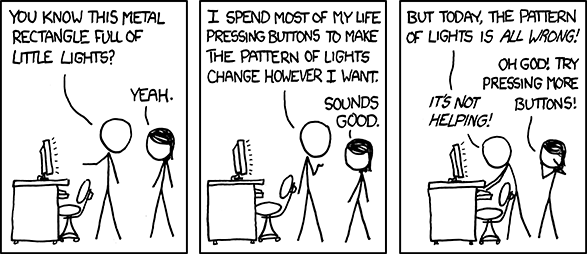
\includegraphics[scale=.5]{img/computer_problems.png}
        \caption{\footnotesize{xkcd.com}}
    \end{figure}
\end{frame}

\backupend

\end{document}
